\section{Mikrofone}
\subsection{Richtcharakteristik}
\textit{"Die Richtcharakteristik definiert, aus welcher Richtung das Mikrofon den Schall besonders empfindlich aufnimmt. Stark vereinfacht gesagt: Aus welcher Richtung aufgenommen wird."}\footnote{\label{}https://www.delamar.de/mikrofon/richtcharakteristik-mikrofon-22647/ [Zugriff: 17.03.2018]} 
\subsubsection[Kugelcharakteristik]{Kugelcharakteristik\protect\footnote{\label{}vgl. https://www.delamar.de/mikrofon/richtcharakteristik-mikrofon-22647/ [Zugriff: 17.03.2018]}}
Bei der Kugelcharakteristik wird der Schall von allen Richtungen aufgenommen, das heißt es wird von keiner bevorzugten Richtung aufgenommen. Das Problem, was dadurch entsteht, ist, dass die Rückkoppelanfälligkeit sehr hoch ist, wodurch Mikrofone mit einer Kugelcharakteristik schlecht für Bühnen geeignet sind. 
%\begin{figure}[H]
%	\centering
%	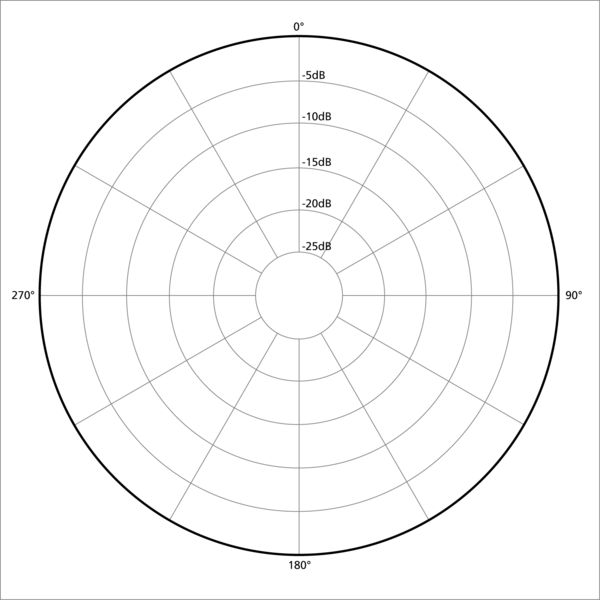
\includegraphics[width=0.4\textwidth]{abb4} 
%	\caption{Kugel}
%\end{figure}
\subsubsection{Nierencharakteristik}
Die Niere nimmt, im Gegensatz zur Kugelcharakteristik, aus einer bevorzugten Richtung auf. Wo, der Schall bei der Kugel von allen Seiten aufgenommen wird, wird er bei der Niere nur von einer Seite aufgenommen, meistens von vorne. Der Schall wird von den Seiten nur sehr leise bis gar nicht aufgenommen. Der Vorteil, der Niere ist, dass sie rückkopplungsfester, als die Kugel ist und sie so auch beispielsweise bei Konzerten verwendet werden kann. Der Nachteil der Niere ist der sogenannte Nachbesprechungseffekt. Das bedeutet: "Ab einer gewissen Nähe der Schallquelle werden die tieffrequenten Anteile dominanter."\footnote{\label{}https://www.delamar.de/faq/nahbesprechungseffekt-34021/ [Zugriff: 17.03.2018]}
%\begin{figure}[H]
%	\centering
%	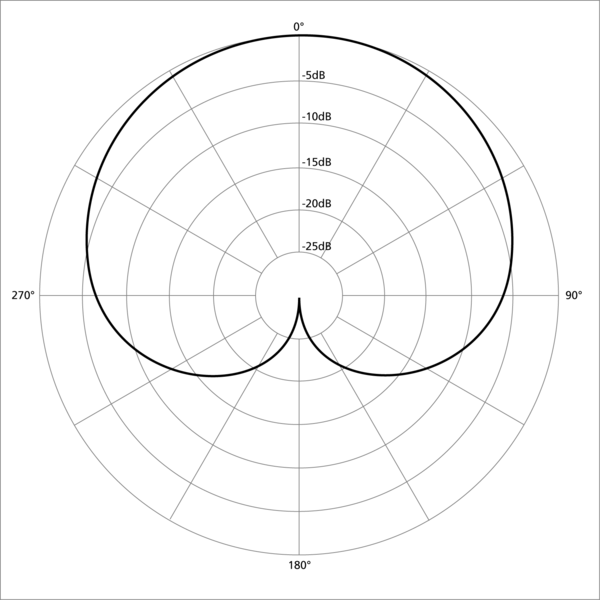
\includegraphics[width=0.4\textwidth]{abb5} 
%	\caption{Niere}
%\end{figure}
\subsubsection{Keule/Superniere}
Keule beziehungsweise Superniere sind Charakteristiken, die von der Niere abgeleitet sind. Die Fläche der Keule ist im Gegensatz zu der Niere etwas schmaler. Das hat die Auswirkung, das von den Seiten weniger aufgenommen wird. Dadurch sind Mikrofone mit einer Keule oder Superniere hinten empfindlicher. "Dennoch haben sie die höchste Rückkopplungsfestigkeit."\footnote{\label{}https://www.delamar.de/mikrofon/richtcharakteristik-mikrofon-22647/ [Zugriff: 17.03.2018]}
%\begin{figure}[H]
%	\centering
%	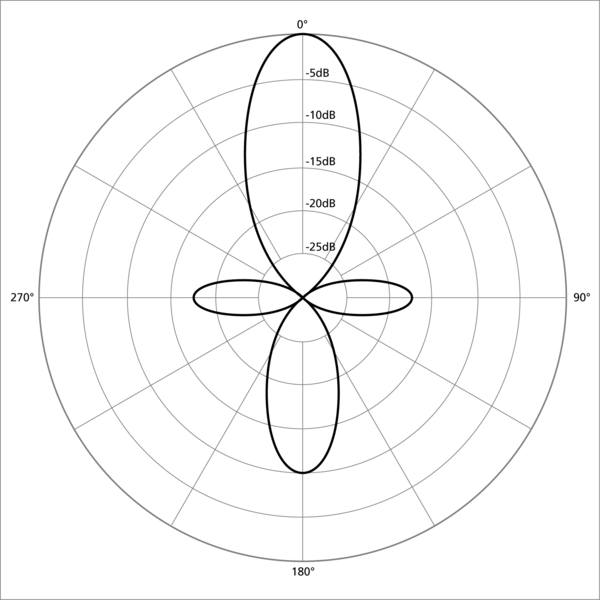
\includegraphics[width=0.4\textwidth]{abb6} 
%	\caption{Keule}
%\end{figure}
\subsubsection{Acht}
Die sogenannte Achtcharakteristik nimmt den Schall von vorne und hinten auf, jedoch nur minimal von den Seiten. Diese Charakteristik hat die Verwendung bei der M/S-Stereofonie. 
%\begin{figure}[H]
%	\centering
%	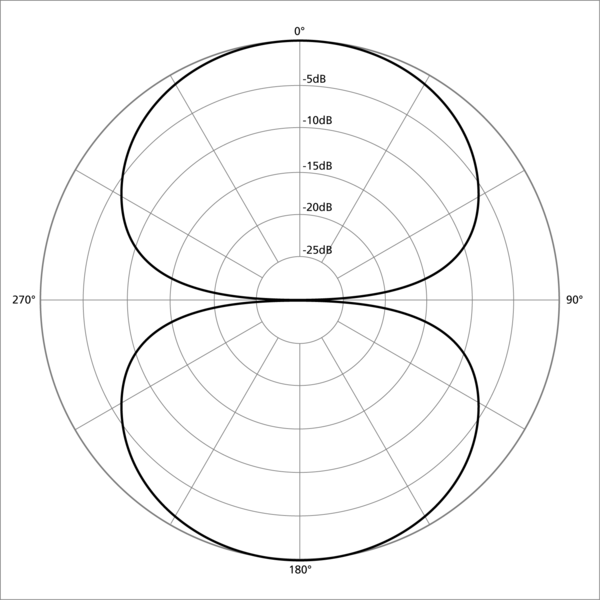
\includegraphics[width=0.4\textwidth]{abb7} 
%	\caption{Acht}
%\end{figure}
\subsection{Kondensatormikrofon}
"Ein Kondensatormikrofon wandelt Schall in ein elektrisches Signal."\footnote{\label{}https://www.delamar.de/faq/kondensatormikrofon-34728/ [Zugriff: 17.03.2018]} Bei einem Kondensatormikrofon treffen die Schallwellen zuerst auf die Membran, was eine leitende Folie ist, die mit Gold bedampft ist. Dies verbessert die  Leitfähigkeit des Mikrofons, was die Luftdruckschwankungen in mechanische Schwingungen umwandelt.\footnote{\label{}vgl. https://www.delamar.de/faq/kondensatormikrofon-34728/ [Zugriff: 17.03.2018]} Anschließend wird sie in elektrische Spannung umgewandelt und über die XLR-Buchse wieder ausgegeben. 
%\begin{figure}[H]
%	\centering
%	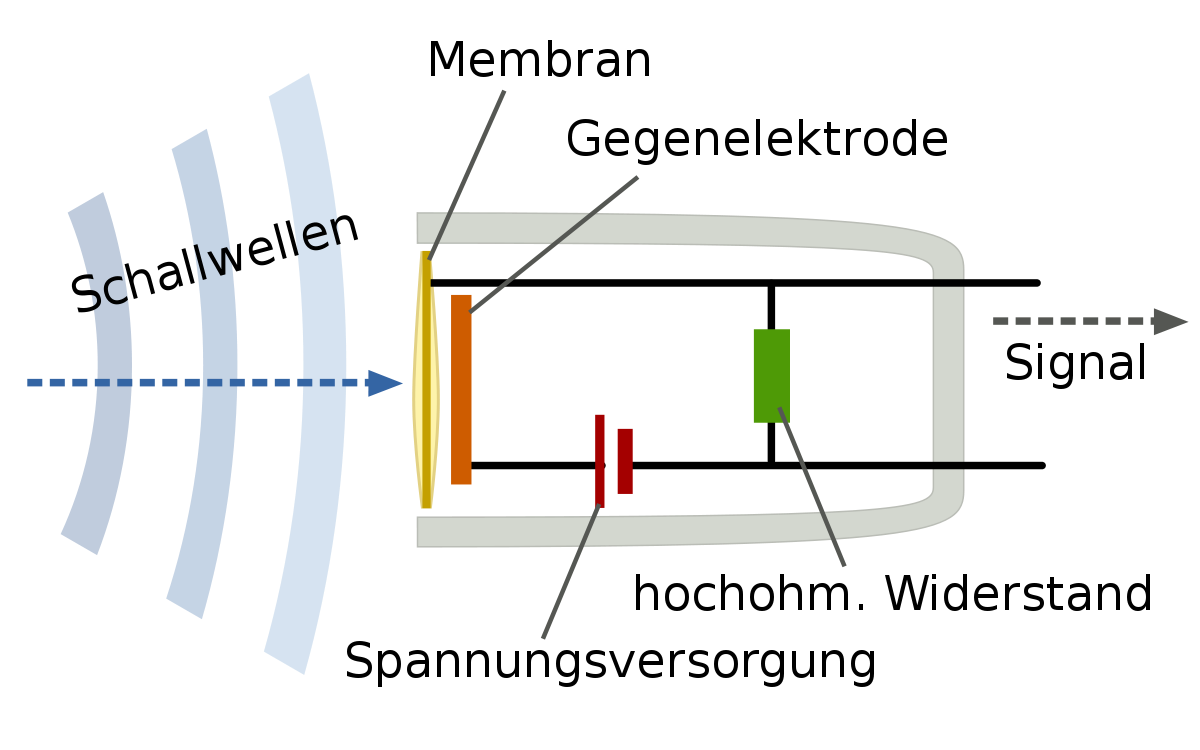
\includegraphics[width=0.6\textwidth]{abb8} 
%	\caption{Kondensatormikrofon}
%\end{figure}
\subsection{Dynamisches Mikrofon}
\textit{"Bei diesem Mikrofontyp wird das Signal durch elektromagnetische Induktion erzeugt. Kurz: Der Schall trifft auf die Membran des Mikrofons und regt sie zu mechanischen Schwingungen an, die durch eine mit der Membran verbundene Spule in elektrische Spannung umgewandelt werden. Und diese kommt dann aus der (XLR-)Buchse des Mikrofons."}\footnote{\label{}https://www.delamar.de/faq/dynamisches-mikrofon-34718/ [Zugriff: 17.03.2018]} \\ \\
%\begin{figure}[H]
%	\centering
%	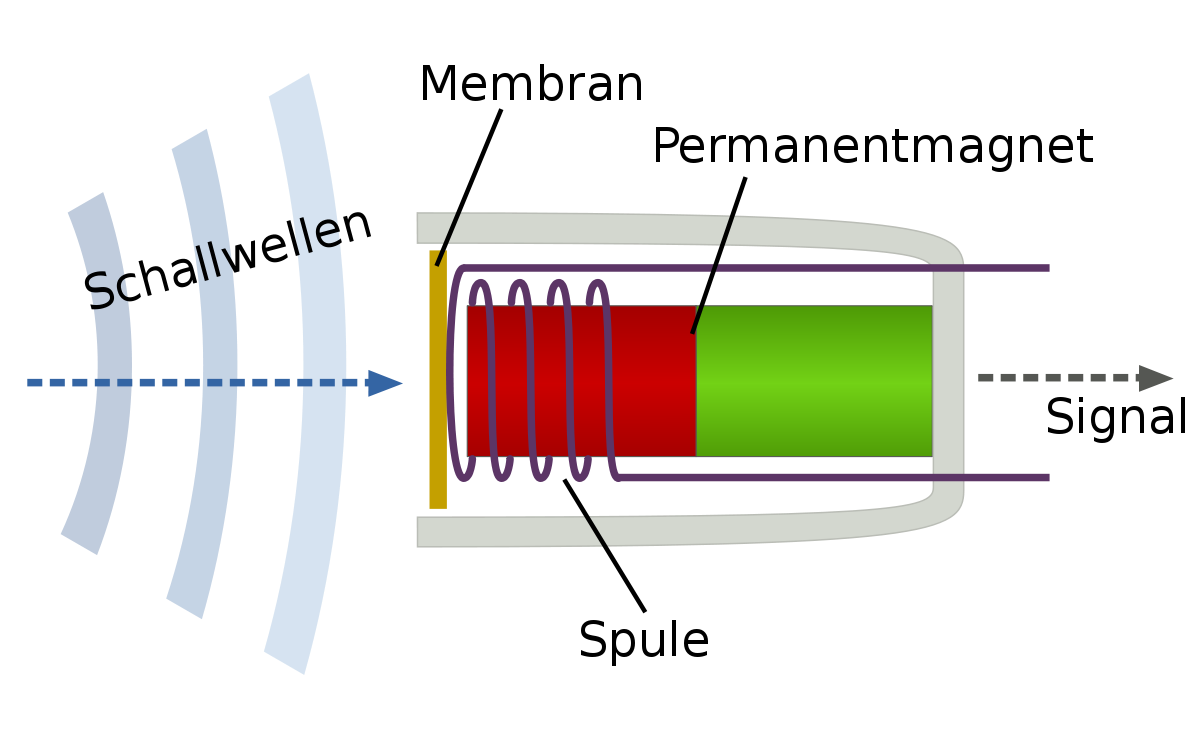
\includegraphics[width=0.6\textwidth]{abb9} 
%	\caption{Dynamisches Mikrofon}
%\end{figure}
Bei dem Dreh des Videos mit dem Abteilungsvorstand Dr. Hager wurde ein Mikrofon mit Kugelcharakteristik verwendet. Das Mikrofon lag in der Mitte des Tisches, um einen natürlichen Effekt zu erzeugen und um von der Interviewerin und dem Interviewten auf einem Mikrofon die Stimmen einfangen zu können.
Bei dem Tag der offenen Tür Video wurde eine Angel für die Interviewten verwendet. Hierfür wurde eine Keule beziehungsweise eine Superniere eingesetzt. Das hat den Vorteil, da beim Interview viel Hintergrundgeräusche vorhanden waren, dass weniger von den Seiten aufgenommen wird, dafür das meiste von vorne.
Beim Quiz mit dem Absolventen und dem Schüler der zweiten Klasse wurde, wie beim ersten Interview, ein Mikrofon mit Kugelcharakteristik verwendet. Dies spiegelte nicht das typischen Interview Bild wieder, da man zum Beispiel die Ansteckmikrofone nicht gesehen hat und es so natürlicher dem Betrachter erscheinen lässt.